\section{Question 1}\label{question-1}

(Credit: Tuomo Tanila)

\subsection{Get all records with search key greater than 40}\label{section}

The tree nodes that must be fetched are: \textbf{I1}, \textbf{I2} as well as every node between \textbf{L2-L8} (that is \textbf{L2, L3, L4, L5, L6, L7} and \textbf{L8}). As we are searching all the records with search key greater than 40, we begin from the top node and choose the lower node that is between 30 and 80, that is \textbf{I2} in this case. After this we choose the node that is between 35 and 42. Finally we get to the leaf nodes and go all of them through.

Note that \textbf{I3} is not visited because leaf nodes are doubly-linked. 


\subsection{Inserting a record with search key 88}\label{section-1}

As there is enough space for the key 88 in the tree, there is no need to additional operations (e.g. splitting leaves) after finding the correct leaf (\textbf{L6}). By inserting the search key \textbf{88*}, we will get the resulting tree in Figure~\ref{fig:q1-1}.

\begin{figure}[H]
  \centering
  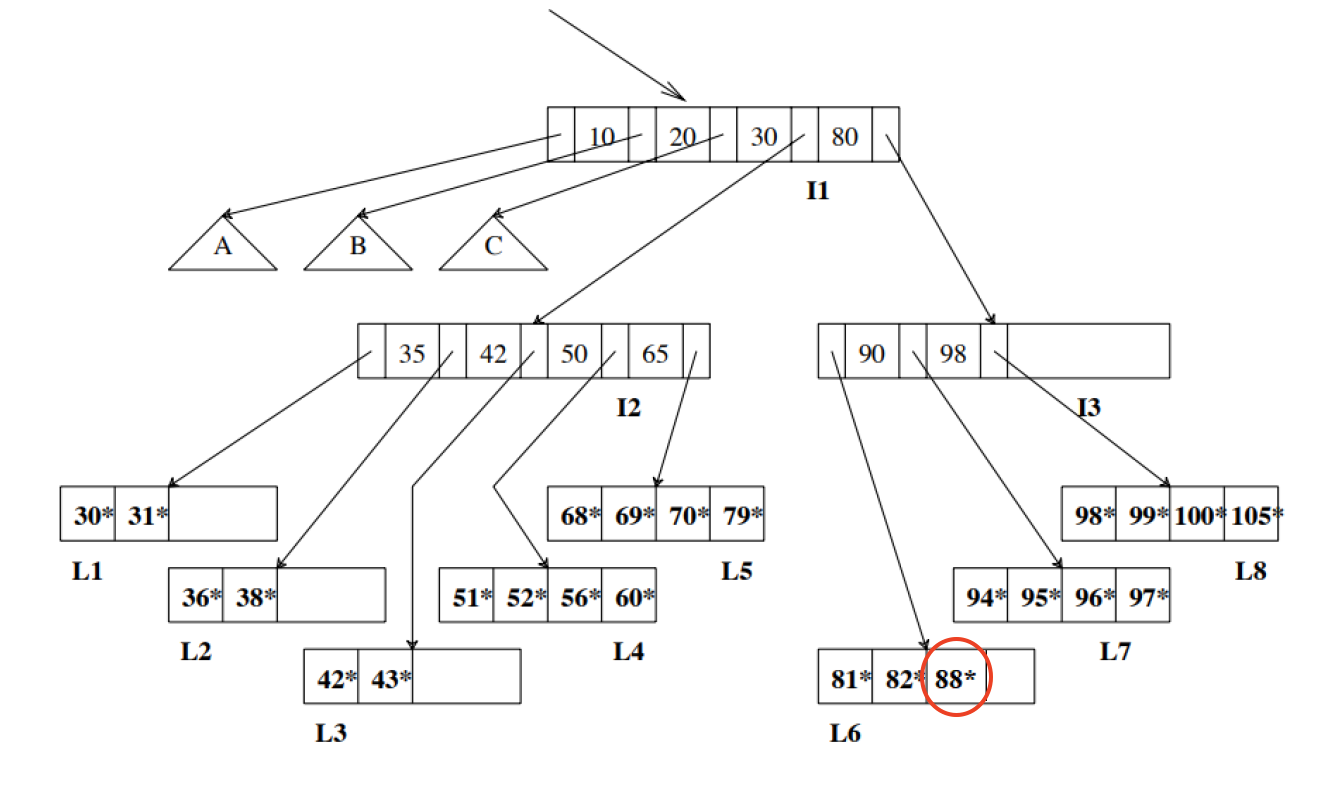
\includegraphics[width=0.9\linewidth]{figs/q1-2.png}
  \caption{B+ tree after inserting search key 88.}
  \label{fig:q1-1}
\end{figure}

\subsection{Inserting a record with search key 109}\label{section-2}

As there is not enough space for the key 109 in the tree, additional operations need to be performed.
The leaf \textbf{L8} will be split into two leaves so that we get a new one (\textbf{L9}).
The leaves are redistributed evenly and middle key is copied to the parent of L8. By inserting the search key \textbf{109*}, we will get the following tree in Figure~\ref{fig:q1-3}.

\begin{figure}[H]
  \centering
  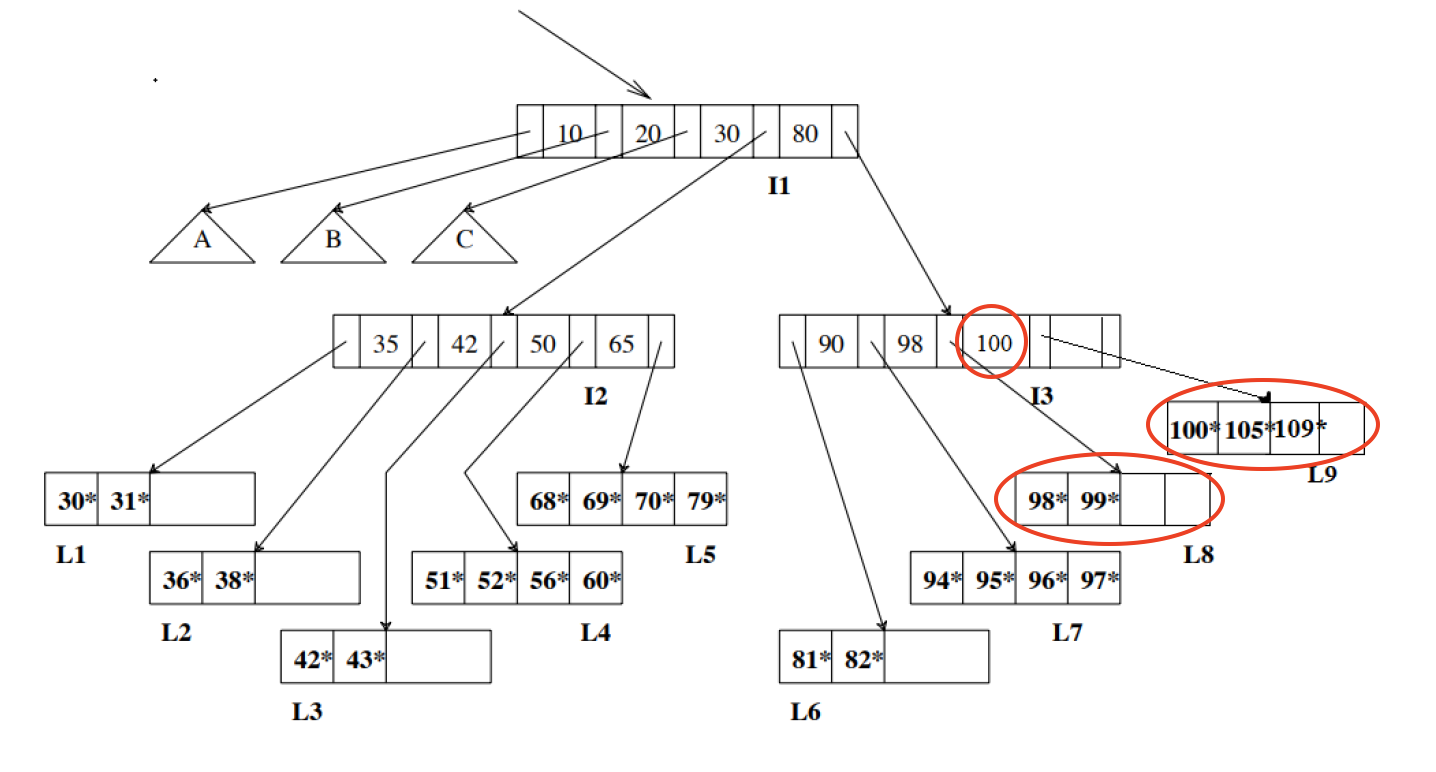
\includegraphics[width=0.9\linewidth]{figs/q1-3.png}
  \caption{B+ tree after inserting search key 109.}
  \label{fig:q1-3}
\end{figure}

\subsection{Contents and shape of subtrees A, B and C}\label{section-3}

\begin{itemize}
  \tightlist   
\item \textbf{tree height}: \textbf{A}, \textbf{B}, \textbf{C} should have the same height as \textbf{I2} and \textbf{I3}
\item \textbf{key range}: for A $[-\infty, 10)$, for B, $[10, 20)$, for C, $[20,30)$
\item \textbf{occupancy}:   each non-leaf node should have at least 2 search key values and 3 pointers while  each leaf node should have at least 2 data entries.
\end{itemize}
  